\documentclass[tikz]{standalone}

\usetikzlibrary{positioning}

\begin{document}
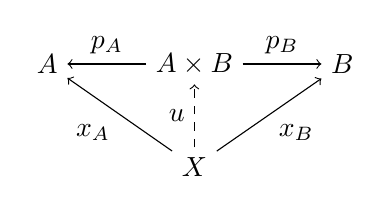
\begin{tikzpicture}
	\node (A) {$A$};
	\node [right=1.0cm of A] (P) {$A\times B$};
	\node [right=1.0cm of P] (B) {$B$};
	\node [below=0.8cm of P] (X) {$X$};
	\draw [->] (P) to node [above] {$p_A$} (A);
	\draw [->] (P) to node [above] {$p_B$} (B);
	\draw [->, dashed] (X) to node [left] {$u$} (P);
	\draw [->] (X) to node [below left] {$x_A$} (A);
	\draw [->] (X) to node [below right] {$x_B$} (B);
\end{tikzpicture}
\end{document}
